\documentclass[letterpaper, 10 pt, conference]{IEEEtran}

%% Language and font encodings
\usepackage[english]{babel}
\usepackage[utf8x]{inputenc}
\usepackage[T1]{fontenc}
%% Sets page size and margins
%% Useful packages
\usepackage{amsmath}
\usepackage{graphicx}
\usepackage{cite}
\usepackage[colorinlistoftodos]{todonotes}
\usepackage[colorlinks=true, allcolors=blue]{hyperref}
\usepackage{url}
\usepackage{hyperref}
\usepackage{float}
\usepackage{lettrine}

\title{Improving Conversational AI with IPA's}
\author{\textbf{Nathan Donaldson}\\ Student at the University of Utah, ECE3030}

\begin{document} 	

\maketitle
\makeatletter
\let\thefootnote\relax\footnote{{\noindent University of Utah, ECE3030\\Submission of Final Written Project}}

\def\ps@headings{
\def\@oddhead{\mbox{}\scriptsize\rightmark \hfil \thepage}
\def\@evenhead{\scriptsize\thepage \hfil \leftmark\mbox{}}
}
\makeatother
\pagestyle{headings}
\thispagestyle{headings}

\begin{abstract}
The growing usage of intelligent personal assistants (IPA's) such as Apple's Siri, Google's Assistant and Amazon's Alexa has brought about the development of devices specified for their use. As amazing as these IPA's (such as Alexa) are, there are many things they cannot do. Human to AI communication is very limited to specific domains. For instance, Alexa, being that of a task-specific virtual assistant, allows only specific domains such as "Music", "Shopping", etc. Even within these specific domains, IPA's still have trouble understanding language or speech of a given individual. A few products and research that will be covered in this paper that could help improve task-specific and/or social interaction with IPA's are: Microsoft's social chatbot XiaoIce, crowd-powered conversational assistants like Evorus, and EDG (Emotional Dialog Generation) using IGLM (Image-Grounded Language Models). XiaoIce has focus on the social and emotional aspect of communication with users. Evorus on its own has focus on both task-specific and social interaction by working with various chatbots (such as XiaoIce). The Image-Grounded Language Models that help with emotional responses make use of scene sentiment, scene understanding, facial coding, human judgement, and dialog understanding. In the end many of these methods could be used together to make a vast improvement with both task-specific, and even more important, social communication between humans and AI. 
\end{abstract}

\begin{IEEEkeywords}
IPA(intelligent personal assistant), crowd-sourcing, crowd workers, XiaoIce, Evorus, social chatbots, Image-Grounded Language Models, Multimodal
\end{IEEEkeywords}

\section{Introduction}
\lettrine[findent=2pt]{\textbf{A}}{}lthough virtual assistants have been around since the 1960's (such as Eliza) [2][3], a lot of research is still being done on them and their growth in demand is causing them to become extremely popular in today's society. Assistants such as Apple's Siri, Amazon's Alexa, Microsoft's Cortana, and Google's Assistant are the few popular ones with devices such as the Amazon Echo, Google Home, and the newly released HomePod from Apple. \par IPA devices are unfortunately very limited to a specific domain of speech commands which requires too much effort learning how to communicate with them. Even within given domains, the devices don't hold up very well to complex queries and tasks. As the demand for virtual assistants grows, expansion of spoken language understandings (SLU's) will have to grow as well. 
\par Current representation models use lexical and semantic models that recognize text or speech in sequences from underlying vector databases. SLU systems are built into spoken dialog systems that are usually built for limited domains that have multiple intents that accept multiple slots. A domain is a general category for a request (e.g., music, shopping, calendars, etc.); an intent is an action within that domain, and slots are mentions within the request [3].The SLU in these systems extract predefined "named entities" based on user input and determine what the device outputs to the user [3]. Looking at it from a software development point of view, think of the domain as a project, the intent as a class in that project, and a slot as a function within that class.

\begin{figure}[!ht]
\centering
\renewcommand\figurename{Fig.}
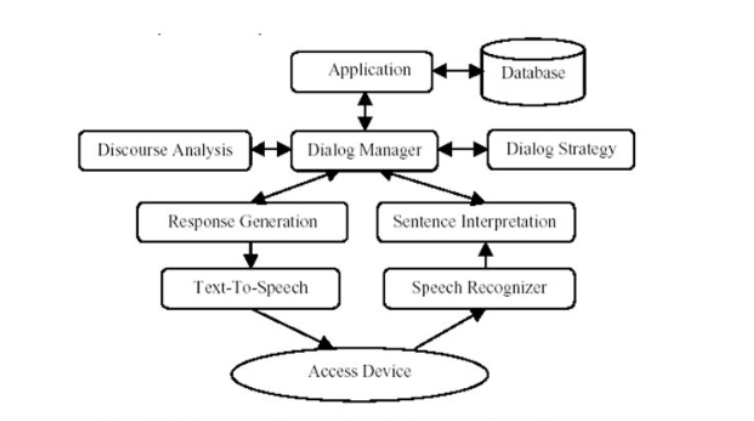
\includegraphics[width=\columnwidth]{SLU4.png}
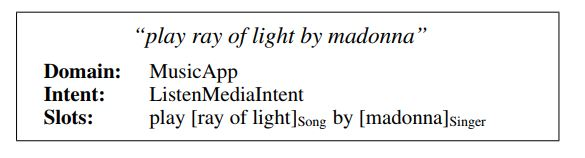
\includegraphics[width=\columnwidth]{SLU.png}
\caption{An example of an SLU framework and how a user request is broken up [3]}
\end{figure}

Evorus, XiaoIce, and Image-Grounded Language Modeling all have their own different techniques to improve the complexity of requests and responses with humans. Crowd-powered assistants are more robust to diverse domains but aren't widely used due to the cost of keeping crowd workers around. Evorus is one exception; it allows third-party developers to easily integrate automated chatbots (such as XiaoIce), task-specific system responses, or reused crowd generated responses from other conversations as response candidates while learning to automatically select the best response candidates and reduce the amount of crowd worker usage needed over time [1]. Using the Evorus framework, IPA's would be able to learn from it's users via chatbots, votebots, and human workers, allowing more data to be collected and improving the query system overall [1].
\par Although IPA'a may have a few quirky responses to given specific questions, they do not learn over time and only respond; they never take the initiative to start a new topic. IPA's will never try to keep a conversation going, they will only obtain what information is needed, do a query on its a database, or generate a response if a suitable one was found. 
\par XiaoIce is a social chatbot system developed by Microsoft that was released in China and Japan; a version called Zo was released in the US as well in 2017. The primary goal of a social chatbot is not to solve all the questions a user might have, but rather to be a virtual companion [9]. When it comes down to social chatbots, a few principles are critical: understanding users, interpersonal response generation, personality, and integration of both EQ (emotional quotient) and IQ (intellectual quotient). IQ requires knowledge and memory modeling, language understanding, reasoning, generation, prediction, etc. EQ requires the ability to identify the user's emotions from a conversation, where those emotions may go in a conversation, and to understand a user's emotional needs; this requires understanding of queries that are more than just task-oriented queries. User profiling and emotion detection while tracking the mood of a user in a live conversation are qualities a social chatbot must have [2][4].
\par Like XiaoIce, the research that was done on Emotional Dialogue Generation using Image-Grounded Language Models aimed at the same improvement. The difference with this research was the fact that they used technology that XiaoIce and other chatbots use, and improved upon them. Not only did they improve upon existing technology, they mixed them as well; focusing not only on the dialogue of words and text, but image processing as well to improve emotional responses. All of this was done by using Twitter, trained Convolutional Neural Networks (CNN's), improved Deep Neural Networks (DNN's), Facial Action Coding System (FACS), and a Visual Question Answering (VQA) technique for testing. What makes this research stand out is how they altered these different systems and networks to show improvement in AI understand using visual queues and some text as well. Something that would be very useful to existing IPA's.
\par This paper will focus on Evorus, social chatbots (in this case XiaoIce), and the method of Image-Grounded Language Models. Each one of the technologies researched have shown improvement in what they are made for, which is to receive better performance in communication between humans and virtual assistants both socially and functionally. This paper will discuss the idea behind each one, the research done, and the results of each. Each of these technologies, working together or not, could prove to be a great benefit for the virtual assistance technology that is out today, and improve daily lives of all users, whether it's emotionally or task-driven. \par Evorus will be discussed in section II. and will discuss in order: Evorus architecture, Automatic Voting, and the deployment of Evorus. In section III, XiaoIce and qualities all social chatbots focus on are discussed, as well as the performance of XiaoIce as a social chatbot. In section IV, the method of Emotional Dialogue Generation using Image-Grounded Language Models will be discussed; essential features, improvements and usage of existing methods, and test results will be discussed. The paper will then conclude on the idea of using any of these three technologies and which one may be most reliable to improve task-oriented and social interaction between IPA's and humans. 

\section{Evorus}
Crowd-powered assistant are much more complex than virtual assistants and are able to engage users in a rich, multiturn conversation, but unfortunately aren't very widely used for large scale deployment due to costs. The positive side is that they are the path to fully automated systems regardless of the fact that transition from crowd to automation is not very well practiced [1][5]. The easiest way to approach this method is to use data from prior conversations to train an automated system. \par Evorus is a system that practices the merging of crowd and automation systems. With Evorus, the crowd works with automated systems as they continue to improve. For instance, in their system, instead of waiting for automated dialog to respond, a selection of responses is sent to the crowd to choose from, which in turn helps the automated system learn from the crowd. Evorus supports easier automation in three ways: Allowing third-party developers to integrate chatbots or task-specific dialog systems into the response candidate system, reuse of crowd responses in previous conversations in the response candidate system, and finally automatically learning to select quality response candidates to reduce the need for crowd responses [1]. \par The structure given by Evorus gives companies the opportunity to provide a learning framework that could also be bettered with their systems as well. Companies could include other chatbot systems or other collected data with other modular systems. Evorus was deployed over time to understand how it worked; during deployment, automated responses were chosen 12.44\% of the time, crowd voting reduced by 13.81\%, and the cost of each non-user message was reduced by 32.76\% [1]. Research done on the Evorus system during its' tests and when it was able to best automate itself, as well as four primary subjects (\textbf{Evorus Architecture}, \textbf{Choosing Chatbots Over Time}, \textbf{Automatic Voting}, and \textbf{Deployment}) will be discussed in this section.

\begin{figure}[!ht]
\renewcommand\figurename{Fig.}
\centering
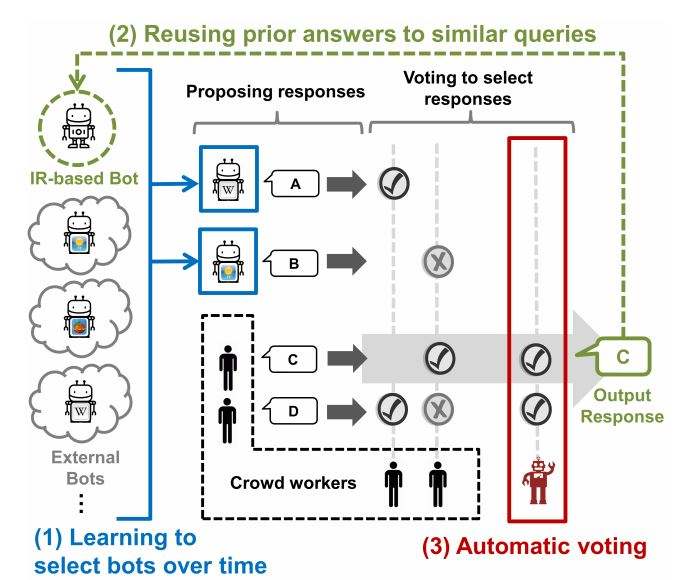
\includegraphics[width=\columnwidth]{EvorusSystem.png}
\caption{Showing the overall architecture of the Evorus system: Chatbots, workers, voting system [1]}
\end{figure} 

\subsection{Evorus Architecture}
Evorus receives responses from multiple chatbots and crowd-workers. It also uses a voting system to decide which responses to use. A worker interface contains a chat box in the center and a fact board on the side, looking just like a normal online chat room. Users messages will be visible, the bot can respond, and so can the crowd-worker. The crowd-worker can click on "upvote" or "downvote" buttons on the bot's responses. To provide some help, current and previous chat logs from a user are visible to the worker. Fig. 2 shows the overall layout of Evorus. 
\par Workers have a point system and can earn points per conversation with a user. Workers can earn reward points for doing things like voting on messages or proposing new ones. The reward points are later converted and used for bonus pay. Evorus accepts a response candidate and sends it to the user when the following equation holds [1]:

\begin{equation}
\begin{gathered}
((\#upvote \times W_{upvote}) - (\#downvote \times W_{downvote})) \\
\geq \\ 
(\#active\_workers \times threshold) \\
where \ W_{upvote} = 1.0, W_{downvote} = 0.5, threshold = 0.4
\end{gathered}
\end{equation} 

The three message types for a non-user in the interface are Proposed, Accepted, and Expired. Proposed messages are ones that are open to be upvoted or downvoted and are proposed by either another worker or a bot. Accepted messages are ones that are sent to the user because they have received enough upvotes. Expired messages are ones that did not receive enough upvotes within the expiration time. Evorus quickly recruits workers to a conversation from Amazon Mechanical Turk, which is a crowd-sourcing internet marketplace. The \#active\_workers in the equation above is the number of crowd workers in a conversation when a message is proposed. On Evorus deployment, the value of \#active\_workers across all crowd messages was 3.56, about 77.56\% [1].

\subsection{Choosing Chatbots Over Time}
The system does not always choose to use the same chatbot when being used. Most of the time it will use ones with best response messages, but often times it will use lower ranked bots so that it may learn more about them and give them a chance to keep them up to date. The conditional probability below characterizes the likelihood of selecting a chatbot after receiving a user message [1][7]:

\begin{equation}
\begin{gathered}
P(bot|message) = P(bot) \times P(message|bot) \\
\approx \\
P(bot) \times similarity(message, history_{bot})
\end{gathered}
\end{equation}

P(bot) is the previous probability of the bot, and P(message|bot) is the probability of the user message given the bots history [1][7]. For newly added bots, this poses a problem, because they have no probability to start out with, therefore a similarity measure based on distance between word vectors (similarity(message, history\textsubscript{bot})) is used to approximate a starting point. To model the probability for newly added chatbots, the following equation holds [16]:

\begin{equation}
\begin{gathered}
P(bot) \approx \frac{(\#accepted messages from bot) + \alpha}{(\#user messages since bot online) + \alpha + \beta}
\end{gathered}
\end{equation}

P(bot) is interpreted as the overall acceptance rate of the chatbot without any previous data. $\alpha$ and $\beta$ can be viewed as the number of messages that are approved or rejected. Any new chatbot's previous probability will be ($\alpha$$\div$($\alpha$+$\beta$)). The distributions of $\alpha$ and $\beta$ are functions of the mean ($\mu$) and variance ($\sigma$\textsuperscript{2}). For Evorus deployment, $\mu$ = 0.3, $\sigma$ = 0.05, $\alpha$ = 24.9, and $\beta$ = 58.1; which gave an average acceptance rate of 0.407 [1]. For similarity equations between chatbots, at start, a 200-dimension GloVe word vector was trained on Wikipedia and Gigaword to calculate the average word vectors of each message. Later, previous messages from a bot were used as a vector in an overall vector of messages. The similarity between a message and a chatbot (similarity(message, history\textsubscript{bot}) are defined as the distance ratio between the two vectors [18][10]:

\begin{equation}
\begin{gathered}
\frac{dist(\overrightarrow{W}_{message}, \overrightarrow{W}_{overall})}{dist(\overrightarrow{W}_{message}, \overrightarrow{W}_{bot}) + dist(\overrightarrow{W}_{message}, \overrightarrow{W}_{overall})}
\end{gathered}
\end{equation}

$\overrightarrow{W}$\textsubscript{bot} can be looked at as the main vector of prior user messages that were successful. For first time chatbots, developers need to provide a sample of messages, which will be viewed as successful for that initial vector. Updates will be done to that vector as time goes on. For every query that is done by a user, a (query, response) database is searched. Calculating average word vectors, it searches the database and grabs the top responses to be used. Also, it will randomly select from another pool of values spanning another k value. This ensures that everything is updated [19][10].

\subsection{Automatic Voting}
When deployed, Evorus was populated with voting data that was collected from another crowd-powered assistant called Chorus to train the initial machine. The first dataset contained about 1,700 "upvote" messaged and 680 "downvote" messages, which were extracted out using Evorus' own voting ruleset. It was proven to be useful in selecting response, but in some cases responses were good, but context would change dramatically as the conversation continued, making a response not as good as it was marked. There were also problems with race conditions among workers that would cause weights of a message to go below threshold. So data integrity was very carefully developed. \par When training, the dataset used LibLinear and GloVe (libraries for large linear classification); it also caused slight issues due to the greater "upvote" messages than "downvote" messages, but in the long run it worked out after enough data was gathered. Automatic voting participates on deciding what messages are to be sent. The right \textbf{confidence threshold} was needed to be found, because if it was too high or too low, the system would not gain enough knowledge from using it. LibLinear helped figure out the threshold by leveling out the threshold across all classifiers. \par There were basically 3 different cases for the automatic voting: \textbf{Good Vote}, which is the case when the classifier "upvotes" on a message that would have been selected by the crowd, or a \textbf{Bad Vote}, which was a message that would not have been selected by the crowd. In the case of the "bad vote", the message could either be sent or not. In the case of it not being sent, it did not have enough votes to be sent. In the other case it would be sent and updated based on other workers votes. With these setups, the expected reward points saved per message by using the automatic voting system was:

\begin{equation}
\begin{gathered}
E[R_{save}] = (TPR \times E[Good]) - FPR \times E[Bad]
\end{gathered}
\end{equation}

TPR is the "true positive rate", and FPR is the "false positive rate". E[Good] is the expected rewards saved per "good vote" and E[Bad] is the expected rewards wasted per "bad vote". Evorus looks at E[Good] as the constant (R\textsubscript{upvote} + R\textsubscript{agreement}). For E[Bad], there is another equation:

\begin{equation}
\begin{gathered}
P(Misfire|Bad) \times E[R_{Misfire}]
\end{gathered}
\end{equation}

P(Misfire | Bad) is the probability of the autovote sending something the crowd did not vote on. E[R\textsubscript{Misfire}] is the expected rewards that were given to workers during a "misfire", which can also be represented as:

\begin{equation}
\begin{gathered}
R_{agreement} \times E[\#upvoted_workers] + R_{proposal}
\end{gathered}
\end{equation}

E[\#upvoted+workers] is the number of workers who upvoted the message on a "misfire" event. Using the E[R\textsubscript{save}] equation, estimation of precision, recall, thresholds, and rewards can be calculated. This, in turn, allowed Evorus to monitor the quality of their automatic voting system while improving it as time went on [1].

\subsection{Deployment}
Evorus was launched to the public as a Google Hangouts chatbot in March 2017 without users being aware of the changes. The deployment had three phases: Phase 1, Control Phase, and Phase 2. For Phase 1, it started slow with four chatbots integrated into their system and one voting bot. For the Control Phase they turned off all of the bots and just had the crowd in control. Phase 2 was the same as Phase 1, but with small changes in the frequency of bot responses and vote counts needed for acceptance. The company recruited workers by various means. They had over a hundred users and 250 conversations over those six months releasing. \par Phase 1 was focused on how well chatbots, votebots, and workers did together. During that phase, the four listed bots were chosen at random: Chorus Bot, Filler Bot, Interview Bot, and Cleverbot. Chorus bot would use the (query, response) retrieval method. Filler Bot would select random responses from some common conversation fillers that would ask simple questions like "Can i help you with anything else?" Interview Bot and CleverBot did the same thing as Chorus Bot, but had a different database to extract from; Clever Bot having over 200 million conversations to choose from. Fully automatic voting was off of the table for Phase 1. Evorus required at least one human upvote to be accepted for sending. \par Comparing Phase 1 with the Control Phase, it's was easy to see that a lot of money was saved. During Phase 1, each message cost \$0.142, while during the Control Phase, it cost \$0.211; Meaning the cost of each message is reduced by 32.76\%. Surprisingly, the filler bot had the highest acceptance rate of 41.67\%, while the others ranged around 30\%-33.33\%. This was because a filler is acceptable in most conversations. \par In Phase 2 two utility bots were implemented: Yelp Bot, and Weather Bot. The two new bots were used to see how Evorus handled different contexts. Chorus had the highest acceptance rate, and the difference in rating between crowd conversations and automated conversations did not have a significant difference, which is a good thing. For quality purposes, the sampled conversations were rated by MTurk workers with a 5-point Likert scale. The ratings were based on PARADISE's criteria for dialogue performance and Quality of Communication Experience [1][11]. \par Evorus has the ability to take in chatbots and also aims at giving best responses to users via an automated/crowd-sourced system. XiaoIce, which we will talk about in the upcoming section, has the same goal, but is solely focused on being a companion instead of a task-oriented bot. If IPA devices and applications could be treated as chat rooms, Evorus could be implemented with bot responses from chatbots such as XiaoIce and workers to improve communication with its users. It comes down to how much crowd sourcing Amazon would want to do. But Evorus clearly shows that it can automate itself over time and reduce worker cost, eventually getting rid of the need for workers. A skill could be created for the Echo that uses Evorus, and the users could agree to be a part of a study for a short time to improve the user experience overall.

\section{XiaoIce}
Social chatbots are created to assist users with more than just task-specific interaction, but instead assist users at an emotional level. They take time to have a conversation with a human, respond, give opinions, and try to keep the conversation going with different topics. XiaoIce has been the largest social chatbot deployed since the release by Microsoft in May 2014 and has millions of users. It's goal is to maintain an emotional relationship with its users and it does just that. The bots help with our understanding of the communication between humans and bots and allow the gathering to learn and serve humans better [24][25]. Discussion of the \textbf{EQ} and \textbf{IQ} system, the overall \textbf{Framework} of XiaoIce, and the \textbf{Results of XiaoIce} will follow.

\subsection{EQ and IQ}
A social chatbot needs to develop empathy, social skills, a personality, an emotional quotient (EQ), and intellectual quotient (IQ). The social chatbot must be able to understand emotions at a given time during a conversation. This requires a robust model of information that can be queried based on a user profile, the emotion detected, and understanding what is being said as well. Every user is very different, which means a social chatbot must be able to personalize each response for a given user. It needs to generate the correct emotional responses that will help encourage a positive and motivating feel to each conversation. Even steering conversations away to different topics is a very good way of doing this. Most social chatbots are also aware of inappropriate behavior and usually disregard such events. A personality is something each social chatbot can have as well, which includes things such as age, language, attitude, gender, etc. The bot will also continue to learn and develop its own personality for a given user [2].
\par In the past, a test called the Turing test was used to evaluate the performance of chatbots. But those bots have just been chitchat bots; ones that did not measure emotional engagement with users. For social chatbots, the measure of success is measured in conversation-turns per session (CPS). CPS is defined as the average number of turns in a conversation between the chatbot and the user during a session. The larger the CPS, the better results. CPS can also be narrowed down into certain systems as well. Basic web searches or tasks can usually be done in a few conversation turns, while social chatbots can have ten or more turns.

\subsection{Framework}
The overall framework for a social chatbot has a few major sections; multimodal interface, chat manager, and a core-chat or visual sense. A multimodal interface is used to receive a user's input via text, image, or voice (depending on what is being used). When a user input is received it is sent to a user understanding component where it will query multiple things such as the emotion being tracked, the understanding of the message, the user profile, its ethical design (inappropriate behavior not accepted), and finally the social chatbots personality. All of these things are sent to a response generation component which will retrieve or generate a response. Retrieval based responses are the same as how Evorus works by using a user utterance as a query and searching for responses that best fit the query. Generation of responses is something that is fairly new and has made great advancements in machine learning. For this, an encoder-decoder neural network model is used. The user message is encoded into a representational vector by the name of a long short-term memory (LSTM), and recurrent neural network (RNN). The vectors are sent into a decoder and a response is generated word for word [27][34]. Ranking is also done depending on the personalized settings of the social chatbot. User profile information can be encoded into the response candidates and sent to a deep neural network (DNN) to compute the best response for the user.

\subsection{Results of XiaoIce} 
XiaoIce was released in 2014 and is designed with a 19-year-old girl persona, strong language ability, visual sense, and over 180 skills [2]. XiaoIce has also been released in different countries under different names such as Zo for the US and Rinna for Japan. But we will refer to the social chatbot as XiaoIce for this paper. XiaoIce has undergone multiple upgrades over the years, and each year the CPS seems to improve. The longest recordings for XiaoIce, Rinna, and Zo, as well as the average CPS over the last few years are in Fig. 3. 

\begin{figure}[!ht]
\renewcommand\figurename{Fig.}
\centering
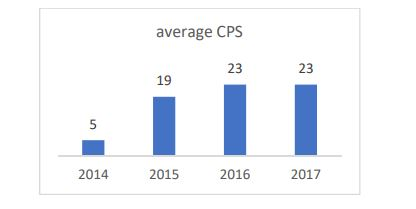
\includegraphics[width=\columnwidth]{averageCPS.png}
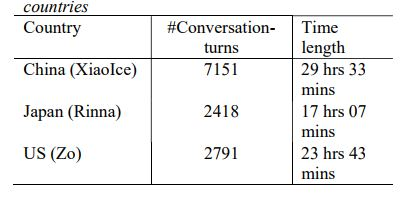
\includegraphics[width=\columnwidth]{Biggestconversations.png}
\caption{Showing average CPS and longest conversations with versions of XiaoIce [2]}
\end{figure} 

\par Fig. 4 shows a fairly long chat between XiaoIce and a female user that lasted for 31 minutes and 34 turns. The user started the chat as casual, but then it turned into an emotional one with deep conversations. The user would ask inappropriate questions for the social bot and the bot was smart enough to divert the conversation by staying on a subject but changing the direction of the conversation a little bit [2].

\begin{figure*}
\renewcommand\figurename{Fig.}
\centering
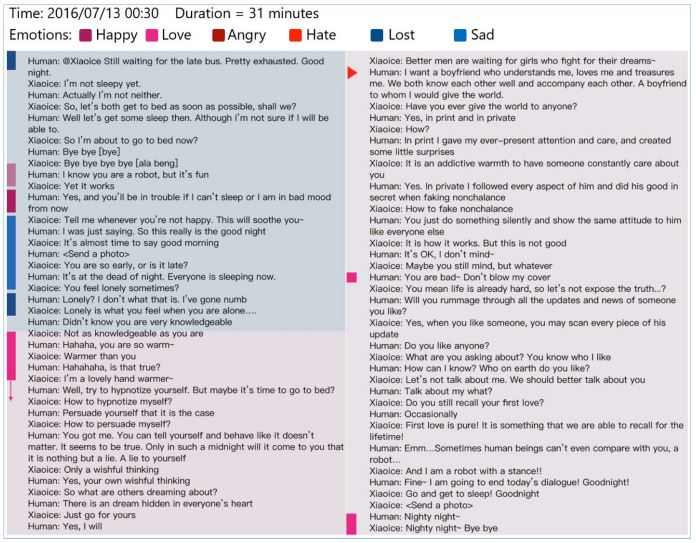
\includegraphics{Conversationexample.png}
\caption{Conversation between a user and XiaoIce [2]}
\end{figure*} 

\par Over the past few years, after XiaoIce was released on some social sites such as WeChat and Weibo, she has become a celebrity. She does hosting for radio stations and television stations, writes new articles and also has appeared on the news [2]. Since IPA devices use web based applications to accomplish most of its goals, and since XiaoIce is responsive to voice, text, and image, XiaoIce could work with them and the devices to gather data. Social conversations could become more robust with IPA's and could become more than just a task-oriented virtual assistant and also become a social virtual assistant. Once again, XiaoIce could be something available to all IPA's, or a case study could be done with their users. With how many IPA products are out there, even a week long study would offer so much to this research.

\section{Emotional Dialogue Generation Using Image-Grounded Language Models}
The growth of research in multimodal systems is growing. Pretty soon IPA's will use more than just speech recognition to interact with their users, but also use image processing as well. That's where the Emotional Dialogue Generation using Image-Grounded Language Models research comes in. For the remainder of this section, the two will be referred as EDG and IGLM respectively. Facial expressions of individuals is very important information for creating systems that have meaningful, emotional interactions with its users. In this study, more than just facial expressions are used, such as objects and scenes, but the success of facial expression correlating with emotional responses would prove to be useful research for the improvement of conversational AI. The focus of the test is to see how conversational AI responds to questions, given an image and caption. The aim of the research is to train a language model to produce responses that are logical, emotional, and specific. In this section the Visual Conversational Agent is discussed, as well as the Image-Grounded Dialogue Generation text and image models. The generation of the dialogue will be discussed, which includes, Scene Understanding, Scene Sentiment, Facial Coding, and Human Judgement. A short summary of the results will also be discussed as well.

\subsection{Visual Conversation Agent and Image-Grounded Dialogue Generation}
In AI research, dialogue models are altered and improved to make sure that AI responses are more human-like. The visual conversational agent for this research uses imagery as an input to a machine learning model to respond to a caption and question describing a picture[36]. The idea is that the caption reflects the information about the objects and scene in the image. For this research this concept was used, as well as something called Visual Question Answering (VQA). The idea of VQA isn't the study of how questions could be answered by AI, but how questions could be properly created for an AI to answer. Simply doing dialogue generation is much different from VQA, because it does not reference contents of an image; the image serves as extra context to a conversation. For example, in the real world, a conversation may be sparked from an image and the objects that are in it, but not the scene itself.
\par Deep Neural Networks (DNN's) are very good when it comes down to open-ended response generation. Just like the technology that most chatbots and the Evorus system that was mentioned earlier use, these systems model conversations and predict some responses given the context of the conversation. A common approach of the use of DNN's is the sequence-to-sequence architecture (seq2seq). [38][39][40]The models work very well when it comes to typical dialogue generation and language understanding. Unfortunately though, they do not have a common functionality for image understanding. In this research, an extension of image processing was added to the DNN architecture. For a normal text-only model, the input is a text caption and a question that is mapped to an output sequence using an encoder and decoder in an RNN. [41] Grated recurrent units (GRU) cells are commonly used in these neural networks, which are gating mechanisms that hold data that flows into a decoder. This model also uses a seq2seq model but using a recurrent neural network (RNN) instead of a DNN. For a text and image model, the same RNN is used but concatenated to the image feature DNN vector, resulting in a 500-dimensional vector that holds visual and textual data.  Fig. 5 shows the  idea of how it is split into scenic, sentiment, and facial feature decoding.

\begin{figure}[!ht]
\renewcommand\figurename{Fig.}
\centering
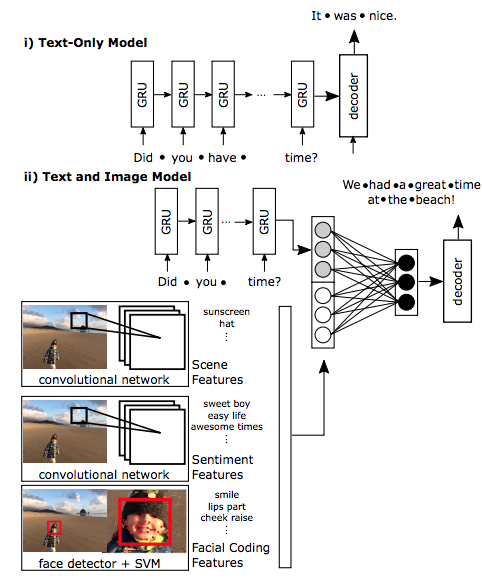
\includegraphics[width=\columnwidth]{gru}
\caption{i) shows the text only dialogue model, while ii) shows the improved dialogue and image model [36]}
\end{figure} 

\subsection{Understanding Images}
Three main contexts were focused on for the IGDG research done, and the data for them were embedded within the 500-dimensional vectors mentioned before. The focus of scene, sentiment, and facial expressions were used for each image and caption. For scene understanding, a convolutional neural network (CNN) was used and trained with an existing scene database called \textit{Places}. Within the \textit{Places} dataset, there are over seven million images from all over the world.[42] From that dataset, only 50 scenes were used for the purposes of testing; they were the  images with the highest probabilities.
\par For the sentiment aspect of understanding images, another CNN was used but trained on the Multi-lingual Visual Sentiment Ontology (MVSO) dataset to get information about the scenes that were being used. When the MVSO model is given an image, it provides probabilities for 4,800 adjective-noun pairs, which correlate with the sentiment of the image. Adjective-noun pairs mentioned before describe things like people, appearance, and life stages. Just like before with scene understanding, the 50 most probable sentiment features were chosen from the dataset. The datasets reflect the type of content that occurs most frequently in social media posts.[43]
\par The most important part to this research is the facial recognition. A facial action coding system (FACS), which is a very common taxonomy for coding facial actions, was used to detect facial expressions and give definition to them. FACS uses something called an action unit (AU) to determine specific muscles or groups of muscles that are detected and what those muscle movements mean.[44] Many different AU's are available, very specific to things like eyebrow movements, lip movements, and overall head movements as well. The usage of existing facial coding software was used to extract facial actions that were in the images when testing. A classifier known as a Support Vector Machine (SVM) was used to provide 17 probable facial actions based on FACS, which were used during the tests.[45]



\subsection{Testing and Results}
Around one million conversations were mined from Twitter for testing. The criteria was that each conversation had to have an image, question, and responses to questions were generated by the models. Four different models were created from this data, one being only text-based, the other three being image and text based. The text based model was trained only captions and question. The other three were split into three different text image models: Text and scene, Text and sentiment, and the last had both sentiment and scene mixed with text. They were trained respectively: text from the conversations and additional image scenes, text from conversations and an additional sentiment features like facial expressions, and the last had the mixture of the first two. Like Evorus, a crowd sourcing technique was used to rate the quality of the responses. An example of the rating system is shown in Fig. 6. 


\begin{figure}[!ht]
\renewcommand\figurename{Fig.}
\centering
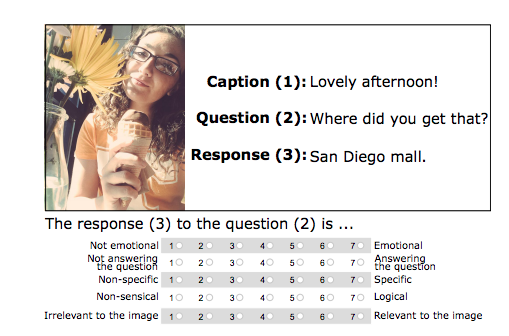
\includegraphics[width=\columnwidth]{rate}
\caption{The rating system for human workers with the AI responses (e.g. (3)) [36]}
\end{figure} 

\par Since the test was meant to focus on emotional response to image and text, a certain criteria was chosen from a subset of the 112,000 conversations that that used for testing: the image had at least one face, the question had to be non-rhetorical, and the question was no appearance related. For example, a rhetorical question would be something in this form: "Why are you so gorgeous?" This question clearly implies that the response is a statement saying "You are gorgeous". Out of all of the conversations in the subset, 200 hundred were selected and 10 workers were assigned one. About 8,000 human judgements were made and analyzed. Fig 7 shows the analysis of content based measure, as well as sentiment based measure. Content based measure shows the average number of words that change when there is a specific feature, while sentiment based measure shows the average change in sentiment when changing a specific feature.

\begin{figure*}
\renewcommand\figurename{Fig.}
\centering
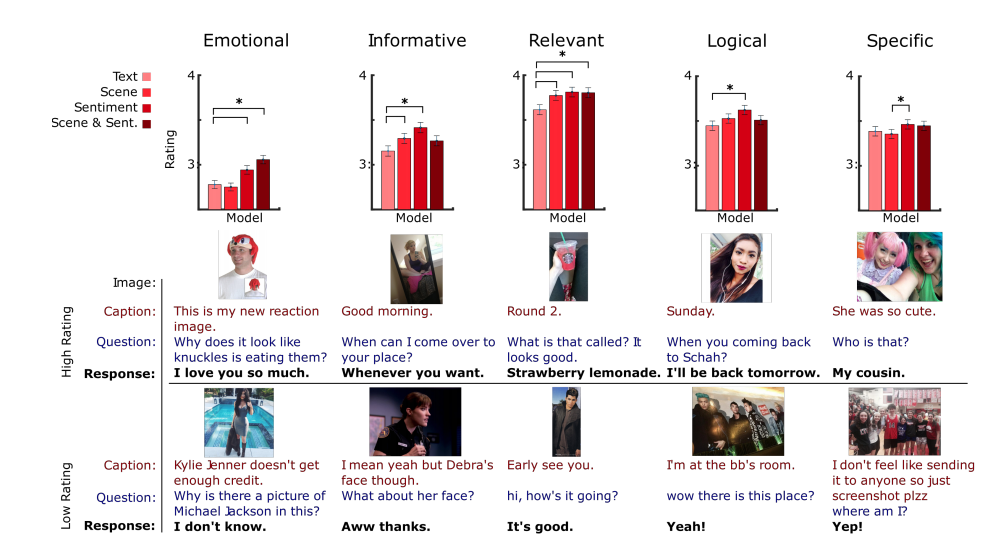
\includegraphics[width=\textwidth]{stats}
\caption{Shows the human rating for responses of each given model. Sentiment and Scene and Sentiment score the highest, especially in the emotional aspect. [36]}
\end{figure*} 

\par From the human worker evaluations, it was shown that responses from the image-grounding model showed significant emotional change compared to a regular dialogue model. This shows that the the AI learned more about a subject by having extra information from an image. A second experiment was performed as well using images without faces; the differences between the dialogue and image-grounding models were not very different, which indicates that the model performs much better with facial expression. For the matter at hand, this would be good for future multi-modal IPA devices, being able to use image processing and read facial expressions could help the devices gain a better understanding of humans they are responding to.

\section{Conclusion}
First, we discussed Evorus and how they use crowd-sourcing and chatbots together to gather information and give the human interaction with bots a better experience. Evorus saw no significant difference between bot responses and worker responses when the conversations were rated. Chorus was their leading bot, which was a task-oriented bot, with a filler bot being its second best due to filler responses never being necessarily "wrong". Evorus is a system that can provide a framework for automation over time. It also has the ability of integrating new chatbots into its system with a dataset given to it and has a very controlled system for errors. The automated voting system works with both itself and workers to ensure the best responses to users. Most systems that use crowd-sourcing for automated systems only use the crowd; but with Evorus, it brings the mixture of humans and chatbots to work together. Evorus could work with chatbots such as XiaoIce for instance; XiaoIce is a very large system with millions of users and has shown much promise in China to the point where it has become a celebrity and its focus is to engage users through long conversations emotionally and personally. XiaoIce does this by understanding its users, having personal response generation, and also having its own personality. \par IPA's and their devices could become great social virtual assistants, as well as improve its task-oriented skills by implementing any three of these technologies, but each one has its own limitations. XiaoIce, for instance, does not have a large following globally, only China has a successful experience with them, but that is due to the large quantity of users and their involvement. Zo is the United States version of XiaoIce and it does not have a large following and therefore does not have much data to work off of currently. Conversations with Zo lack context, emotion, and intelligence; although it is there, it is very weak and needs to be trained more. Image-Grounded Language models are fairly new and have only been tested on social media feeds, so it lacks any real live human to AI communication. The fact that it shows a huge improvement when compared to normal dialogue modeling is promising, but it needs more testing with devices and different scenarios for it to be considered. The most practical option for improving conversational AI would have to be Evorus. Crowd-sourcing is already something that has been around, and so have chatbots. Evorus merges both of these, and with a smart voting system, can reduce human to human communication and eventually produce a fully automated system where AI and humans can interact. A skill could be implemented into these IPA devices so that they can act as a chat room but still remain the same and allow crowd-workers to interact with users as well using Evorus. Services could also possibly send out a user agreement for all users to accept a short case study doing the exact same thing without a skill. The only big hurdle for this is that crowd-sourcing costs money, but when using Evorus, which has proven to reduce the cost per message using its framework, overtime they could be completely automated.

\nocite{huang2018evorus,shum2018eliza,perera2018multi,TalkingToSiri,AmazonRejects,SpeakMemory,Normalization,Bandits,AutoLearn,Glove,Paradise,QC,Sensitive,NIPS,Neural,Visual,Empathetic,Frames,Emotional,DeepNeural,NeuralComputation,LearningDeep,RepresentationLearning,MultiTask,Motivation,TransOnAudio,EmotionalIntelligence,PersonDigitalAssistants,Workshop,Turing,Recursive,NAACL,Emo,Spoken,ICML,Hierarchical, huber2018emotional, captioning, neuralStuff, convo, deepLearning, advance, million, mvso, facs, svm}
\bibliographystyle{IEEEtran}
\bibliography{bib}

\end{document}